% Compiling with
% latexmk -halt-on-error -shell-escape -synctex=1 -pdf maths.tex
% (Recommend using a latexmkrc file so as just to run latexmk -pvc, for example)
% Probably you can achieve the same with an inordinate number of invocations of
% pdflatex -halt-on-error -shell-escape -synctex=1 maths.tex

% fleqn aligns equations to the left, a4 paper size, 11pt font, article class
\documentclass[fleqn,a4paper,11pt]{article}
\title{IA Vectors and Matrices Example Sheet 2}
\author{Izaak van Dongen (\texttt{imv26})}

\usepackage{mymaths}
\usepackage{mystyle}

\begin{document}
 \maketitle\thispagestyle{empty} % no page number under title

 \begin{enumerate}[label=\textbf{\arabic*.}]
  \item
   \begin{enumerate}[label=(\alph*)]
    \item \(
     \begin{aligned}[t]
      \delta_{ij} v_j &= v_i \\
      \delta_{ij} \delta_{jk} &= \delta_{ik} \\
      \delta_{ij} \delta_{ji} &= \delta_{ii} = 3 \\
      \delta_{ij} v_i v_j &= v_j v_j = \abs{\vec v}^2 = \vec v \vecdot \vec v \\
      \epsilon_{ijk} \delta_{jk} &= \epsilon_{ikk} = 0 \\
      \epsilon_{ijk} v_j v_k &=  (\vec v \veccross \vec v)_i = 0 \\
                  \text{or,} &= -\epsilon_{ikj} v_{j} v_{k}
                              = -\epsilon_{ijk} v_{j} v_{k},
                              \quad
                              \text{relabelling. So
                                    \(\epsilon_{ijk} v_j v_k = 0\).} \\
      \epsilon_{ijk} \epsilon_{ij\ell} &= 2\delta_{k\ell} \\
      \epsilon_{ijk} \epsilon_{ikj} &= - \epsilon_{ijk} \epsilon_{ijk}
                                     = -6,
                                     \quad
                                     \text{as 6 of the possible combinations are
                                           permutations.}
     \end{aligned} \)
    \item \(
     \begin{alignedat}[t]2
      && A_{ij} &= \epsilon_{ij\ell} a_\ell \\
      \implies{}&&
         \epsilon_{ijk} A_{ij} &= \epsilon_{ijk} \epsilon_{ij\ell} a_\ell \\
         &&                    &= 2\delta_{k\ell} a_\ell \\
         &&                    &= 2 a_k \ (\Forall k)
     \end{alignedat} \)
    \item For some \(k\), the expression \(\epsilon_{ijk} S_{ij}\) evaluates to
          \(S_{ij} - S_{ji}\) where \(i\), \(j\) are the two indices other than
          \(k\) such that \(ijk\) is an even permutation. But then immediately,
          \(\epsilon_{ijk} S_{ij} = 0 \Forall k \implies
            S_{ij} - S_{ji} = 0 \implies
            S_{ij} = S_{ji} \Forall i \ne j\) as each of the choices of
          \(k\) gives one of the choices of distinct pairs of \(i\), \(j\).
          The only cases not covered are non-distinct pairs, which just give the
          trivial statement \(S_{ii} = S_{ii}\).

          Similarly,
          \(S_{ij} = S_{ji} \Forall i, j \implies
            S_{ij} - S_{ji} = 0 \Forall i \ne j \implies
            \epsilon_{ijk} S_{ij} = 0 \Forall k\)
          picking \(k\) to be the remaining index that is not \(i\) or \(j\).
   \end{enumerate}
  \item \(
   \begin{aligned}[t]
    \epsilon_{ijk} (\vec a \veccross \vec b)_k
     &= \epsilon_{ijk} \epsilon_{mnk} a_m b_n \\
     &= (\delta_{im} \delta_{jn} - \delta_{in} \delta_{jm}) a_m b_n \\
     &= a_i b_j - b_i a_j
   \end{aligned} \)

   So
   \begin{align*}
    (\vec c \veccross (\vec a \veccross \vec b))_i
     &= \epsilon_{ijk} c_j (\vec a \veccross \vec b)_k \\
     &= c_j (a_i b_j - b_i a_j) \\
     &= (c_j b_j) a_i - (c_j a_j) b_i \\
     &= (\vec c \vecdot \vec b) a_i - (\vec c \vecdot \vec b) b_i \\
     &= ((\vec c \vecdot \vec b)\,\vec a - (\vec c \vecdot \vec b)\,\vec b)_i
   \end{align*}
   and therefore
   \(\vec c \veccross (\vec a \veccross \vec b) =
     (\vec c \vecdot \vec b)\,\vec a - (\vec c \vecdot \vec b)\,\vec b\).
   \begin{enumerate}[label=(\alph*)]
    \item \(
     \begin{alignedat}[t]2
      && \vec r \veccross \vec u &= \vec m \\
      \implies{}&& \vec a \veccross (\vec r \veccross \vec u)
       &= \vec a \veccross \vec m \\
      \implies{}&& (\vec a \vecdot \vec u)\,\vec r -
                   (\vec a \vecdot \vec r)\,\vec u &= \vec a \veccross \vec m \\
      \implies{}&& (\vec a \vecdot \vec u)\,\vec r -
                   \kappa\,\vec u &= \vec a \veccross \vec m \\
      \implies{}&& \vec r &=
                   \frac{\vec a \veccross \vec m + \kappa\,\vec u}
                        {\vec a \vecdot \vec u}
                   \quad
                   \text{as \(\vec a \vecdot \vec u \ne 0\).} \\
     \end{alignedat} \)

     Then we can check that
     \begin{align*}
      \vec r \vecdot \vec a
       &= \frac{0 + \kappa\,\vec u \vecdot \vec a}
               {\vec a \vecdot \vec u} \\
       &= \kappa
     \end{align*}
     and
     \begin{align*}
      \vec r \veccross \vec u
       &= \frac{(\vec a \veccross \vec m) \veccross \vec u + \vec 0}
               {\vec a \vecdot \vec u} \\
       &= \frac{\vec u \veccross (\vec m \veccross \vec a)}
               {\vec a \vecdot \vec u} \\
       &= \frac{(\vec u \vecdot \vec a)\,\vec m - (\vec u \vecdot \vec m)\,\vec a}
               {\vec a \vecdot \vec u} \\
       &= \frac{(\vec u \vecdot \vec a)\,\vec m - 0 \cdot \vec a}
               {\vec a \vecdot \vec u} \\
       &= \vec m
     \end{align*}
     Geometrically, the condition \(\vec a \vecdot \vec u \ne 0\) means that the
     direction vector of the line is not perpendicular to the normal of the
     plane, ie the line is not parallel to the plane, so there is a unique point
     of intersection.
    \item
     We have \(\vec a, \vec b \in  \Reals^3\) with
     \(\vec a \veccross \vec b \ne \vec 0\), meaning \(\vec a\) and \(\vec b\)
     are linearly independent. But then
     \begin{alignat*}2
      && (\vec r \vecdot \vec a = \kappa \quad &\text{and} \quad
          \vec r \vecdot \vec b = \rho) \\
      \iff{}&& (\vec r \vecdot \vec b)\,\vec a - (\vec r \vecdot \vec a)\,\vec b
       &= \rho\,\vec a - \kappa\,\vec b
       \quad \text{due to linear independence} \\
      \iff{}&& \vec r \veccross (\vec a \veccross \vec b)
       &= \rho\,\vec a - \kappa\,\vec b
     \end{alignat*}
     If \(\vec a \veccross \vec b = \vec 0\), then:
     \begin{itemize}
      \item
       If \(\vec a = \vec b = \vec 0\), there exist solutions only if
       \(\kappa = \rho = 0\), and then the solutions are \(\Reals^3\).
      \item
       If \(\vec a = \vec 0\), there exist solutions only if
       \(\kappa = 0\), and then the solutions are the plane
       \(\vec r \vecdot \vec b = \rho\).
      \item
       If \(\vec b = \vec 0\), there exist solutions only if
       \(\rho = 0\), and then the solutions are the plane
       \(\vec r \vecdot \vec a = \kappa\).
      \item
       Otherwise, we have that the normals to the two planes are parallel, so
       the planes are parallel. They have an intersection only if
       \(\kappa / \abs{\vec a} = \rho / \abs{\vec b}\), and then this
       intersection is the entirety of either plane.
     \end{itemize}
   \end{enumerate}
  \item
   If \(\mat M_{ij} = \delta_{ij} + \epsilon_{ijk} n_k\),
   \(\mat N_{ij} = \delta_{ij} - \epsilon_{ijk} n_k + n_i n_j\), and
   \(n_i n_i = 1\), then
   \begin{align*}
    \mat N_{ij} \mat M_{jk}
     &= (\delta_{ij} - \epsilon_{ij\ell} n_\ell + n_i n_j)
        (\delta_{jk} + \epsilon_{jkq} n_q) \\
     &= \delta_{ik} + \epsilon_{ikq} n_q
        - \epsilon_{ik\ell} n_\ell
        - \epsilon_{ij\ell} \epsilon_{jkq} n_\ell n_q
        + n_i n_k + \epsilon_{jkq} n_q n_i n_j \\
     &= \delta_{ik} + \epsilon_{ik\ell} n_\ell
        - \epsilon_{ik\ell} n_\ell
        - \epsilon_{ij\ell} \epsilon_{jkq} n_\ell n_q
        + n_i n_k \\
     &= \delta_{ik}
        - \epsilon_{j\ell i} \epsilon_{jkq} n_\ell n_q
        + n_i n_k \\
     &= \delta_{ik}
        - (\delta_{k\ell}\delta_{iq} - \delta_{q\ell}\delta_{ik}) n_\ell n_q
        + n_i n_k \\
     &= \delta_{ik}
        - n_i n_k + \delta_{ik} n_\ell n\ell
        + n_i n_k \\
     &= \delta_{ik}
        + \delta_{ik} \cdot 1 \\
     &= 2\delta_{ik}
   \end{align*}
   so
   \begin{alignat*}2
    && (\mat N \mat M)_{ik} &= 2\delta_{ik} \\
    \implies{}&& \mat N \mat M &= 2\mat I
   \end{alignat*}
   If
   \begin{alignat*}2
    && \vec y &= \vec x + \vec x \veccross \vec n \\
    \iff{}&& y_i &= x_i + (\vec x \veccross \vec n)_i \\
    &&           &= x_i + \epsilon_{ijk} x_j n_k \\
    &&           &= \delta_{ij} x_j + \epsilon_{ijk} x_j n_k \\
    &&           &= \mat M_{ij} x_j
   \end{alignat*}
   So then \(\vec y = \mat M \vec x \implies
    \vec x = \mat M^{-1} \vec y = \frac 12 \mat N \vec y\), ie
   \begin{align*}
    2 x_i &= \mat N_{ij} y_j \\
          &= (\delta_{ij} - \epsilon_{ijk} n_k + n_i n_j) y_j \\
          &= y_i - \epsilon_{ijk} y_j n_k + n_i(\vec n \vecdot \vec y) \\
          &= y_i - (\vec y \veccross \vec n)_i + n_i(\vec n \vecdot \vec y)
   \end{align*}
   and
   \(2\,\vec x
     = \vec y - \vec y \veccross \vec n + (\vec n \vecdot \vec y) \vec n\).
   \item
    Any set of 5 vectors in \(\Reals^4\) is linearly dependent as
    \(\Reals^4\) has dimension \(4\). So it will be sufficient to find two
    subsets that are linearly independent, of size \(4\).
    \begin{itemize}
     \item
      We claim
      \(\set{\vec a_1 = (1, 1, 0, 0),\ \vec a_2 = (0, 0, 1, 1),
           \ \vec a_3 = (1, 0, 0, 1),\ \vec a_4 = (1, 0, 1, 0)}\)
      is such a set. Note that
      \(\vec e_1 = \frac 12 (\vec a_3 + \vec a_4 - \vec a_2)\), and therefore
      immediately we can express each standard basis vector in terms of this
      set:
      \(\vec e_2 = \vec a_1 - \vec e_1\),
      \(\vec e_3 = \vec a_4 - \vec e_1\),
      \(\vec e_4 = \vec a_3 - \vec e_1\).

      So this set spans \(\Reals^4\). It must therefore be linearly independent.
     \item
      Similarly,
      \(\set{\vec b_1 = (1, 1, 0, 0),\ \vec b_2 = (0, 0, 1, 1),
           \ \vec b_3 = (1, 0, 0, 1),\ \vec b_4 = (0, 1, 0, 1)}\)
      is such a set. Note that
      \(\vec e_4 = \frac 12 (\vec a_3 + \vec a_4 - \vec a_1)\), and therefore
      \(\vec e_1 = \vec a_3 - \vec e_4\),
      \(\vec e_2 = \vec a_4 - \vec e_4\),
      \(\vec e_3 = \vec a_2 - \vec e_4\).

      So this set spans \(\Reals^4\). It must therefore be linearly independent.
    \end{itemize}
   \item
    Use the check that for a vector space \(V\), a nonempty subset \(U \in V\)
    is a subspace iff
    \\ \((\vec v, \vec w \in U \implies \lambda \vec v + \mu \vec w \in U)\) for
    all scalars \(\lambda\), \(\mu\).

    Note that \(\vec 0 \in V\).

    Have \(\vec v, \vec w \in V\). Let \(\vec x = \lambda \vec v + \mu \vec w\)
    for arbitrary \(\lambda, \mu \in \Reals\). Now for any \(i\),
    \begin{align*}
     x_i &= (\lambda \vec v + \mu \vec w)_i \\
         &= \lambda v_i + \mu w_i \\
     \intertext{and therefore,}
     x_i + x_{i + 1} + x_{i + 2} + x_{i + 3} &=
      \lambda(v_i + v_{i + 1} + v_{i + 2} + v_{i + 3}) +
      \mu(w_i + w_{i + 1} + w_{i + 2} + w_{i + 3}) \\
      &= 0 + 0 = 0
    \end{align*}
    and \(\vec x\) is indeed in \(V\).

    Note that any vector in \(V\) necessarily has the form
    \begin{equation*}
     (a, b, c, -(a + b + c), a, b, c, -(a + b + c), \dotsc)
    \end{equation*}
    ie the first three components can be freely chosen but then the rest are all
    determined by the rule (and are in fact periodic).

    Then it is fairly clear that \(V\) is isomorphic to \(\Reals^3\) and
    \begin{align*}
     \{&\vec e_1' =
        (1, 0, 0, -1, 1, 0, 0, -1, \cdots), \\
       &\vec e_2' =
        (0, 1, 0, -1, 0, 1, 0, -1, \cdots), \\
       &\vec e_3' =
        (0, 0, 1, -1, 0, 0, 1, -1, \cdots)\}
    \end{align*}
    forms a basis for \(V\), generating the previously laid out general element
    by \(a\,\vec e_1' + b\,\vec e_2' + c\,\vec e_3'\).
   \item
    The Cauchy-Shwarz inequality states that for
    \(\vec u, \vec v \in \Reals^n\),
    \(\abs{\vec u \vecdot \vec v} \le \abs{\vec u} \abs{\vec v}\).
    Equality holds iff \(\vec u \parallel \vec v\), ie
    \(\vec u = \lambda \vec v\) or \(\vec v = \lambda \vec u\) for some
    \(\lambda \in \Reals\).

    This also implies that
    \(\vec u \vecdot \vec v \le \abs{\vec u} \abs{\vec v}\),
    possibly with equality if \(\vec u \parallel \vec v\), though we need to
    then check the sign of \(\vec u \vecdot \vec v\).
    \begin{enumerate}[label=(\alph*)]
     \item \(
      \begin{alignedat}[t]2
       && (x, y, z) \vecdot (y, z, x) \le \abs{(x, y, z)} \abs{(y, z, x)} \\
       \implies{}&& xy + yz + xz \le x^2 + y^2 + z^2
      \end{alignedat} \)

      with equality iff \(x = y = z\).
     \item Consider
      \begin{align*}
       &\begin{pmatrix}
        x \\ y \\ z \\ 2
       \end{pmatrix} \vecdot
       \begin{pmatrix}
        2 \\ x \\ y \\ z
       \end{pmatrix} +
       \begin{pmatrix}
        x \\ y \\ z \\ 2
       \end{pmatrix} \vecdot
       \begin{pmatrix}
        z \\ 2 \\ x \\ y
       \end{pmatrix} +
       \begin{pmatrix}
        x \\ y \\ z \\ 2
       \end{pmatrix} \vecdot
       \begin{pmatrix}
        y \\ z \\ 2 \\ x
       \end{pmatrix} \\
       &= 4(x + y + z) + 2(xy + yz + xz) \\
       &\le 3(x^2 + y^2 + z^2 + 2^2)
      \end{align*}
      applying Cauchy-Shwarz to each dot product. So \\
      \(3(x^2 + y^2 + z^2 + 4) - 2(xy + yz + xz) - 4(x + y + z) \ge 0\),
      with equality iff \emph{all} of the respective inequalities used are
      equalities.

      Examining the first term (noting neither vector is \(\vec 0\) due to the
      \(2\) component, so the left is \(\lambda\) times the right for some
      nonzero \(\lambda \in \Reals\)), we get
      \(x = 2\lambda = \lambda^2 z = \lambda^3 y = \lambda^4 x\). \(x\) is
      nonzero as we need \(\frac x\lambda = 2\), so \(\lambda^4 = 1\), and
      therefore \(\lambda^2 = 1\) (as \(\lambda^2 > 0\)) and \(x = z\), and
      \(y = 2\).

      But by following the same argument in the third term (for some possibly
      different scalar), \(x = y\) and \(z = 2\). So then the only possible
      solution is \(x = y = z = 2\), which does in fact cause equality to hold
      in all three terms, and therefore satisfies the required equation.
    \end{enumerate}
   \item
    \begin{enumerate}[label=(\alph*)]
     \item \(
      \begin{aligned}[t]
       T: \vec x \mapsto \vec x'
        &= \vec x - (\vec x \vecdot \vec n)\,\vec n \\
        &= (\vec n \vecdot \vec n)\,\vec x - (\vec x \vecdot \vec n)\,\vec n \\
        &= \vec n \veccross (\vec x \veccross \vec n)
      \end{aligned} \)

      So \(\Ker T\) is the set of \(\vec x\) for which
      \(\vec x \veccross \vec n\) is parallel to \(\vec n\),
      which is the set of \(\vec x\) for which \(\vec x \veccross \vec n\) is
      \(\vec 0\), which is the set of \(\vec x\) for which
      \(\vec x \parallel \vec n\), ie
      \(\set{\lambda\,\vec n : \lambda \in \Reals}\).

      Clearly \(\vec x' \perp \vec n\). \(\Img T\) is in fact precisely the
      plane through \(\vec 0\) perpendicular to \(\vec n\). Indeed, consider
      two vectors \(\vec a\), \(\vec b\) spanning this plane
      (so \(\vec a \vecdot \vec n = \vec b \vecdot \vec n = 0\)). Then for any
      \(\alpha, \beta \in \Reals\),
      \(T(\alpha\,\vec a + \beta\,\vec b)
        = \alpha T(\vec a) + \beta T(\vec b)
        = \alpha\,\vec a + \beta\,\vec b \),
      so any point in this plane can certainly be reached by \(T\).
     \item
      \(Q: \vec x \mapsto \vec x' = \vec n \veccross \vec x\)

      \(\Ker Q\) is again the set of all \(\vec x \parallel \vec n\),
      ie \(\set{\lambda\,\vec n : \lambda \in \Reals}\).

      \(\Img Q\) is again the plane perpendicular to \(\vec n\) through
      \(\vec 0\). Let \(\vec m_0\) be some unit normal to \(\vec n\), and let
      \(\vec m_\theta\) denote the unit normal in the plane perpendicular to
      \(\vec n\) making an angle of \(\theta\) with \(\vec m_0\), in the sense
      so that \(\vec n \veccross \vec m_0 = \vec m_{\frac \pi 2}\). Then any
      \(r\,\vec m_\theta = Q(r\,\vec m_{\theta - \frac \pi 2})\), giving a polar
      co-ordinate system spanning the plane perpendicular to \(\vec n\), so each
      point in this plane can be reached by \(Q\).
    \end{enumerate}
    \begin{align*}
     T^2 : \vec x \mapsto T(\vec x')
      &= \vec x' - (\vec x' \vecdot \vec n)\,\vec n \\
      &= \vec x - (\vec x \vecdot \vec n)\, \vec n -
         ((\vec x - (\vec x \vecdot \vec n)\, \vec n) \vecdot \vec n)\,\vec n \\
      &= \vec x - (\vec x \vecdot \vec n)\, \vec n -
         ((\vec x \vecdot \vec n) -
          (\vec x \vecdot \vec n)(\vec n \vecdot \vec n))\,\vec n \\
      &= \vec x - (\vec x \vecdot \vec n)\, \vec n -
         0 \cdot \vec n \\
      &= T(\vec x)
    \end{align*}
    T ``collapses'' all vectors into the plane perpendicular to \(\vec n\) by
    removing the component of \(\vec x\) that is parallel to \(\vec n\),
    somewhat analogously to the reflection map
    \(H: \vec x \mapsto \vec x - 2 (\vec x \vecdot \vec n)\,\vec n\). So \(T\)
    should obviously be idempotent, as once this component has been removed,
    removing it again does nothing.
    \begin{align*}
     Q^2: \vec x \mapsto Q(\vec x')
      &= \vec n \veccross \vec x' \\
      &= \vec n \veccross (\vec n \veccross \vec x) \\
      &= (\vec n \vecdot \vec x)\,\vec n - (\vec n \vecdot \vec n)\,\vec x \\
      &= (\vec n \vecdot \vec x)\,\vec n - \vec x \\
     Q^3: \vec x \mapsto Q^2(\vec x')
      &= (\vec n \vecdot (\vec n \veccross \vec x') - \vec x' \\
      &= -\vec x' \\
      &= - \vec n \veccross \vec x \\
      &= \vec x \veccross \vec n \\
      &= -Q(\vec x)
    \end{align*}
    So \(Q^2 = -T\). Under \(Q^2\), \(\vec x\) is sent to the plane perpendicular
    to \(\vec n\) as with \(T\), but is then inverted through the origin.

    \(Q^3 + Q\) is the null map, and clearly
    \(Q^2 = -T \implies Q^4 = (-T) \circ (-T) = T^2 = T\)
   \item
    \begin{enumerate}[label=(\alph*)]
     \item \(
      \begin{aligned}[t]
       T : (x, y, z) &\mapsto (x + 2y + z, x + 2y + z, 2x + 4y + 2x) \\
                     &= (x + 2y + z)(1, 1, 2)
      \end{aligned} \)

      So \(T\) really only has one degree of freedom, which is along
      \((1, 1, 2)\). \((x + 2y + z)\) can vary over all of \(\Reals\), so the
      image of \(T\) is the span of \((1, 1, 2)\), ie the line
      \(\set{\vec r = \lambda (1, 1, 2)}\).

      The kernel of \(T\) is the set of \(\vec r = (x, y, z)\) for which
      \(x + 2y + z = 0 \iff \vec r \vecdot (1, 2, 1) = 0\). This is the plane
      through \(\vec 0\) perpendicular to \((1, 2, 1)\).
     \item \(
      \begin{aligned}[t]
       S: (x, y, z) &\mapsto (x + 2y + 3z, x - y + z, x + 5y + 5z) \\
                    &= (x + 2y + 3z)(1, 0, 2) + (x - y + z)(0, 1, -1)
      \end{aligned} \)

      Say we let \(y = z\). Then \(x + 2y + 3z = x + 5y\) and \(x - y + z = x\),
      so we can vary both ``parameters'' over all of \(\Reals\), by picking
      \(x\) freely to set the second parameter, and then picking \(y = z\)
      freely to adjust the first parameter. So \(\Img Q\) is the plane spanned
      by \((1, 0, 2)\) and \((0, 1, -1)\), which you could write as
      \(\set{\alpha (1, 0, 2) + \beta (0, 1, -1) : \alpha, \beta \in \Reals}\)
      or
      \begin{align*}
       &\set{\vec r : \vec r \vecdot ((1, 0, 2) \veccross (0, 1, -1)) = 0} \\
       &= \set{\vec r : \vec r \vecdot (-2, 1, 1) = 0} \\
       &= \set{(x, y, z) : -2x + y + z = 0}
      \end{align*}
      For \(Q(\vec r)\) to be \(\vec 0\), we need \(x + 2y + 3z = 0\) and
      \(x - y + z = 0\), as \((1, 0, 2)\) and \((0, 1, -1)\) are linearly
      independent. The set of vectors for which this is true is the intersection
      of the planes with normals \((1, 2, 3)\) and \((1, -1, 1)\), which we
      showed earlier is
      \(\set{\vec r : \vec r \veccross
                      ((1, 0, 2) \veccross (0, 1, -1)) = \vec 0}
        = \set{\vec r : \vec r \veccross (-2, 1, 1) = \vec 0}\).
    \end{enumerate}
   \item
    If \(\mat M \vec r = \vec 0\), then
    \begin{alignat*}2
     && \begin{pmatrix}
      a & a & b & a \\
      a & a & b & 0 \\
      a & b & a & b \\
      a & b & a & 0
     \end{pmatrix}
     \begin{pmatrix}
      x \\ y \\ z \\ w
     \end{pmatrix}
      &= \vec 0 \\
     \iff{}&& \begin{pmatrix}
      0 & 0 & 0 & a \\
      a & a & b & 0 \\
      0 & 0 & 0 & b \\
      a & b & a & 0
     \end{pmatrix}
     \begin{pmatrix}
      x \\ y \\ z \\ w
     \end{pmatrix}
      &=
      \begin{pmatrix}
       aw \\ ax + ay + bz \\ bw \\ ax + by + az
      \end{pmatrix}
      = \vec 0
    \end{alignat*}
    so:
    \begin{itemize}
     \item If either of \(a, b\) is not \(0\), then \(w = 0\), and \(x, y, z\)
           satisfy
      \begin{align*}
       ax + ay + bz &= 0 \\
       ax + by + az &= 0
      \end{align*}
      which is to say \((x, y, z)\) lies on the intersection of the planes
      \(\vec r' \vecdot (a, a, b) = 0\) and
      \(\vec r' \vecdot (a, b, a) = 0\) (where \(\vec r' = (x, y, z)\)).
      \begin{itemize}
       \item
        If \(a = b\), this is the entire plane
        \(\vec r' \vecdot (1, 1, 1) = 0\).
       \item
        Otherwise, these two normal vectors cannot be parallel and this is the
        line \\
        \(\vec r \veccross ((a, a, b) \veccross (a, b, a)) = \vec 0\).
      \end{itemize}
     \item If \(a = b = 0\), then the kernel is \(\Reals^4\).
    \end{itemize}
    For the image:
    \begin{itemize}
     \item
      If \(a = b = 0\), the image is \(\set{\vec 0}\).
     \item If \(a = 0\), the image is the span of
      \(\set{(0, 0, b, b), (b, b, 0, 0), (0, 0, b, 0)}\), which is the span of
      \(\set{(0, 0, 1, 1), (1, 1, 0, 0), (0, 0, 1, 0)}\), as \(b \ne 0\). These
      are linearly independent as all combinations of
      \((0, 0, 1, 1)\) and \((1, 1, 0, 0)\) have the form
      \((\alpha, \alpha, \beta, \beta)\), so can never give rise to
      \((0, 0, \gamma, 0)\). The image is therefore a three-dimensional subspace
      of \(\Reals^4\).
     \item If \(a\) is nonzero, then the image is the span of
      \(\set{(a, a, a, a), (a, a, b, b), (b, b, a, a), (a, 0, b, 0)}\).
      But \(((a + b)/a)\,(a, a, a, a) = (a, a, b, b) + (b, b, a, a)\) is then a
      nontrivial linear dependence, so the image is just the span of
      \(\set{(a, a, b, b), (b, b, a, a), (a, 0, b, 0)}\).

      The linear combinations of \((a, a, b, b)\) and
      \((b, b, a, a)\) have the form
      \begin{equation*}
      (\alpha a + \beta b, \alpha a + \beta b,
       \alpha b + \beta a, \alpha b + \beta a)
      \end{equation*}
      These could only ever give rise to \((\gamma a, 0, \gamma b, 0)\) if
      \begin{align*}
       \alpha a + \beta b &= 0 \\
       \alpha b + \beta a &= 0
      \end{align*}
      has nonzero solutions for \(\alpha, \beta\). Equivalently, there are
      nonzero solutions to
      \begin{equation*}
       \begin{pmatrix}
        a & b \\
        b & a
       \end{pmatrix}
       \begin{pmatrix}
        \alpha \\ \beta
       \end{pmatrix}
       = \vec 0
      \end{equation*}
      so we need \(a^2 - b^2 = 0\). So:
      \begin{itemize}
       \item
        If \(\abs a \ne \abs b\), then the image is the three dimensional
        subspace which is the span of
        \(\set{(a, a, b, b), (b, b, a, a), (a, 0, b, 0)}\).
       \item
        If \(a = b\), then the image is the span of
        \(\set{(a, a, a, a), (a, a, a, a), (a, 0, a, 0)}\), which is the span of
        \(\set{(1, 1, 1, 1), (1, 0, 1, 0)}\) as \(a \ne 0\). This is a plane in
        \(\Reals^4\).
       \item
        If \(a = -b\), then the image is the span of
        \(\set{(a, a, -a, -a), (-a, -a, a, a), (a, 0, -a, 0 )}\), which is the
        span of
        \(\set{(1, 1, -1, -1), (1, 0, -1, 0)}\), again as \(a \ne 0\). This is a
        plane in \(\Reals^4\).
      \end{itemize}
    \end{itemize}
   \item
    If \(\vec n = (0, 0, 1)\), then
    \begin{alignat*}2
     && x_i' &= \cos \theta\,x_i + \delta_{i3} x_3(1 - \cos \theta) -
                \sin \theta\,(\vec x \veccross \vec n)_i \\
     &&      &= \cos \theta\,x_i + \delta_{i3} x_3(1 - \cos \theta) -
                \sin \theta\,\epsilon_{ij3}x_j \\
     \implies{}&& \vec x'
      &=
      \begin{pmatrix}
       \cos\theta\,x_1 - \sin\theta\,x_2 \\
       \cos\theta\,x_2 + \sin\theta\,x_1 \\
       \cos\theta\,x_3 + x_3(1 - \cos\theta)
      \end{pmatrix} \\
     && &=
      \begin{pmatrix}
       \cos\theta\,x_1 - \sin\theta\,x_2 \\
       \sin\theta\,x_1 + \cos\theta\,x_2 \\
       x_3
      \end{pmatrix}
    \end{alignat*}
    as expected.
    \begin{alignat*}2
     && \mat R_{ij} x_j &= x_i' \\
     && &= \cos\theta\,x_i + (\vec x \vecdot \vec n)(1 - \cos\theta)\,n_i
           - \sin\theta\,(\vec x \veccross \vec n)_i \\
     && &= \delta_{ij} \cos\theta\,x_j + x_j n_j (1 - \cos\theta)\,n_i
           - \sin\theta\,\epsilon_{ijk}x_j n_k \\
     \implies{}&&
      \mat R_{ij} &= \delta_{ij} \cos\theta + (1 - \cos\theta)\,n_j n_i
                     - \sin\theta\,\epsilon_{ijk}n_k
    \end{alignat*}
    So
    \begin{align*}
     \mat R_{ii} &= \delta_{ii} \cos\theta + (1 - \cos\theta)\,n_i n_i
                    - \sin\theta\,\epsilon_{iik}n_k \\
      &= 3\cos \theta + 1 - \cos \theta - 0 \\
      &= 2 \cos \theta + 1 \\
     \epsilon_{ijk} \mat R_{jk}
      &= \epsilon_{ijk} (\delta_{jk} \cos \theta + (1 - \cos \theta)\,n_j n_i
                         - \sin\theta\,\epsilon_{jk\ell} n_\ell) \\
      &= \epsilon_{ijk} \delta_{jk} \cos \theta +
          \epsilon_{ijk} (1 - \cos \theta)\,n_j n_i -
          \epsilon_{ijk} \sin\theta\,\epsilon_{jk\ell} n_\ell \\
      &= - \epsilon_{ijk} \sin\theta\,\epsilon_{jk\ell} n_\ell \\
      &= - 2\delta_{i\ell} \sin\theta\,n_\ell \\
      &= - 2 \sin\theta\,n_i
    \end{align*}
    The matrix
    \begin{equation*}
     \mat R = \frac 13
     \begin{pmatrix*}[r]
      2 & -1 & 2 \\
      2 & 2 & -1 \\
      -1 & 2 & 2
     \end{pmatrix*}
    \end{equation*}
    has \(R_{ii} = 2\), so assuming that it is a rotation matrix,
    \(\cos \theta = \frac 12\). Also,
    \begin{equation*}
     \epsilon_{1jk} R_{jk} = \epsilon_{2jk} R_{jk} = \epsilon_{3jk} R_{jk}
      = (-1 - 2) \tfrac 13 = -1
    \end{equation*}
    so \(\sin\theta\,n_i = \frac 12\). Take \(\theta \in \intco{0, \pi}\)
    \footnote{
    The other solution for \(\theta\) gives the same normal but simply inverted.
    }, so
    \(\theta = \frac 13 \pi\) and \(\sin\theta = \frac 12 \sqrt 3\). Then
    \(n_i = \frac 13 \sqrt 3\), so we have a rotation by \(\frac 13 \pi\)
    radians about the unit normal \(\frac 13 \sqrt 3(1, 1, 1)\).
   \item
    \begin{enumerate}[label=(\alph*)]
     \item
      \begin{enumerate}[label=(\roman*)]
       \item \(
        \begin{pmatrix*}[r]
         -1 & 0 \\
         0 & 1
        \end{pmatrix*} \)
       \item \(
        \begin{pmatrix*}[r]
         2 & 0 \\
         0 & 2
        \end{pmatrix*} \)
       \item \(
        \begin{pmatrix*}[r]
         1 & 1 \\
         0 & 1
        \end{pmatrix*} \)
       \item \(
        \begin{pmatrix*}[r]
         1 & -1 \\
         1 & 1
        \end{pmatrix*} \)
      \end{enumerate}
      \begin{itemize}
       \item
        \begin{itemize}
         \item
          The examples I have given show that reflection and
          dil(at)?ation do not necessarily have determinant 1.

         \item
          However, the general form of a rotation is
          \begin{equation*}
           \begin{pmatrix*}[r]
            \cos \theta & -\sin \theta \\
            \sin \theta & \cos \theta
           \end{pmatrix*}
          \end{equation*}
          indeed having determinant \(\cos^2 \theta + \sin^2 \theta = 1\).

         \item
          The general form of a shear parallel to \(\vec i\) with
          factor \(\lambda\) axis is
          \begin{equation*}
           \mat S(\vec i, \lambda)
            =
            \begin{pmatrix*}[r]
             1 & \lambda \\
             0 & 1
            \end{pmatrix*}
          \end{equation*}
          which has determinant 1. This is the general form because in two
          dimensions a unit vector's perpendicular is determined up to sign,
          which is irrelevant as \(\lambda\) can be negative.

          A shear parallel to any other unit vector
          \(\vec n = (\cos \theta, \sin \theta)\) can be expressed
          as a conjugate of this shear by the rotation \(\mat R(\theta)\):
          \begin{equation*}
           \mat S(\vec n, \lambda)
            = \mat R(\theta) \mat S(\vec i, \lambda) \mat R(\theta)^{-1}
          \end{equation*}
          This then clearly also has determinant 1.
        \end{itemize}
       \item
        \begin{itemize}
         \item
          Reflection need not be commutative. Consider reflecting the point
          \((1, 1)\) in the lines \(y = 0\) and \(y = x\). If we reflect in
          \(y = x\) first it ends up at \((1, -1)\), but if we reflect in
          \(y = 0\) first it ends up at \((-1, 1)\).

         \item
          Dilation is commutative. In general,
          \begin{equation*}
           \begin{pmatrix}
            \alpha_1 & 0 \\
            0 & \beta_1
           \end{pmatrix}
           \begin{pmatrix}
            \alpha_2 & 0 \\
            0 & \beta_2
           \end{pmatrix}
           =
           \begin{pmatrix}
            \alpha_1 \alpha_2 & 0 \\
            0 & \beta_1 \beta_2
           \end{pmatrix}
           =
           \begin{pmatrix}
            \alpha_2 & 0 \\
            0 & \beta_2
           \end{pmatrix}
           \begin{pmatrix}
            \alpha_1 & 0 \\
            0 & \beta_1
           \end{pmatrix}
          \end{equation*}
         \item
          Two shears parallel to \(\vec i\) always commute:
          \begin{equation*}
           \begin{pmatrix}
            1 & \lambda \\
            0 & 1
           \end{pmatrix}
           \begin{pmatrix}
            1 & \mu \\
            0 & 1
           \end{pmatrix}
           =
           \begin{pmatrix}
            1 & \lambda + \mu \\
            0 & 1
           \end{pmatrix}
           =
           \begin{pmatrix}
            1 & \mu \\
            0 & 1
           \end{pmatrix}
           \begin{pmatrix}
            1 & \lambda \\
            0 & 1
           \end{pmatrix}
          \end{equation*}
          Then by expressing two shears parallel to some \(\vec n\) as
          conjugates, their commutativity follows.

          Suppose we have the unit vectors
          \(\vec n \nparallel \vec m\), defining the shears
          \(\mat S(\vec n, \lambda)\), \(\mat S(\vec m, \mu)\) where at least
          one of \(\lambda\), \(\mu\) is nonzero. Without loss of generality,
          take \(\mu \ne 0\). Then supposing these shears are commutative,
          \begin{alignat*}2
           && \mat S(\vec m, \mu) \mat S(\vec n, \lambda)
            &= \mat S(\vec n, \lambda) \mat S(\vec m, \mu) \\
           \implies{}&&
            \mat S(\vec m, \mu) \mat S(\vec n, \lambda)\,\vec n
            &= \mat S(\vec n, \lambda) \mat S(\vec m, \mu)\,\vec n \\
           \implies{}&&
            \mat S(\vec m, \mu)\,\vec n
            &= \mat S(\vec n, \lambda) \mat S(\vec m, \mu)\,\vec n
          \end{alignat*}
          So \(\mat S(\vec m, \mu)\,\vec n\) is an eigenvector of
          \(\mat S(\vec n, \lambda)\). But this is only possible if
          \(\mat S(\vec m, \mu)\,\vec n \parallel \vec n\), which is impossible
          since by definition \(\mat S(\vec m, \mu)\) will add some nonzero
          component of \(\vec m\) to \(\vec n\), and
          \(\vec m \nparallel \vec n\).
         \item
          Two rotations always commute.
          \begin{align*}
           &\begin{pmatrix*}[r]
            \cos \theta & -\sin \theta \\
            \sin \theta & \cos \theta
           \end{pmatrix*}
           \begin{pmatrix*}[r]
            \cos \phi & -\sin \phi \\
            \sin \phi & \cos \phi
           \end{pmatrix*} \\
           &=
           \begin{pmatrix*}[r]
            \cos \theta \cos \phi - \sin \theta \sin \phi
             & -\sin \theta \cos \phi - \sin \phi \cos \theta  \\
            \sin \theta \cos \phi + \sin \phi \cos \theta
             & \cos \theta \cos \phi - \sin \theta \sin \phi
           \end{pmatrix*} \\
           &=
           \begin{pmatrix*}[r]
            \cos(\theta + \phi) & -\sin(\theta + \phi) \\
            \sin(\theta + \phi) & \cos(\theta + \phi)
           \end{pmatrix*} \\
           &=
           \begin{pmatrix*}[r]
            \cos \phi & -\sin \phi \\
            \sin \phi & \cos \phi
           \end{pmatrix*}
           \begin{pmatrix*}[r]
            \cos \theta & -\sin \theta \\
            \sin \theta & \cos \theta
           \end{pmatrix*}
          \end{align*}
        \end{itemize}
      \end{itemize}
     \item \(
      \begin{aligned}[t]
       x_1' + ix_2'
        &= (a + ib)(x_1 + ix_2) \\
        &= ax_1 - bx_2 + i(ax_2 + bx_1)
      \end{aligned} \)

      So \(x_1' = ax_1 - bx_2\) and \(x_2' = bx_1 + ax_2\), and then
      \begin{alignat*}2
       && \mat M \vec x = \vec x' &=
       \begin{pmatrix}
        ax_1 - bx_2 \\ bx_1 + ax_2
       \end{pmatrix} \\
       \implies{}&& \mat M &=
       \begin{pmatrix*}[r]
        a & -b \\
        b & a
       \end{pmatrix*}
      \end{alignat*}
      A reflection cannot be represented by a complex number in this way, as a
      reflection generally requires a difference of sign on the leading
      diagonal, and no difference of sign on the trailing diagonal (and they
      can't all be \(0\)):
      \begin{equation*}
       \begin{pmatrix*}[r]
        \cos 2\theta & \sin 2\theta \\
        \sin 2\theta & -\cos 2\theta
       \end{pmatrix*}
      \end{equation*}

      A dilation that scales by the same factor \(k\) in every direction is
      represented by the real number \(k\). A dilation that does not do this
      cannot be represented as the elements of the leading diagonal must be the
      same.

      A non-degenerate shear cannot be represented,
      as then we could make a shear parallel to \(\vec i\) by taking the
      conjugate as discussed earlier, which would also be
      represented by a complex number (see next paragraph).
      But both elements of the trailing diagonal must have the same modulus, but
      for this shear one must be zero and one must be nonzero.

      A rotation by an angle \(\theta\) is represented by
      \(e^{i\theta} = \cos \theta + i \sin \theta\).
    \end{enumerate}
   \item
    \begin{enumerate}[label=(\alph*)]
     \item
      \(\mat R(\vec i, \frac \pi 2)_{ij}
        = \delta_{ij} \cdot 0 + (\vec i)_i (\vec i)_j (1 - 0)
           - \epsilon_{ijk} (\vec i)_k
        = \delta_{i1} \delta_{j1} - \epsilon_{ijk} \delta_{k1}\), so
      \begin{equation*}
       \mat R(\vec i, \tfrac \pi 2)
        =
        \begin{pmatrix*}[r]
         1 & 0 & 0 \\
         0 & 0 & -1 \\
         0 & 1 & 0
        \end{pmatrix*}
      \end{equation*}
      \(\mat R(\vec j, \frac \pi 2)_{ij}
        = \delta_{ij} \cdot 0 + (\vec j)_i (\vec j)_j (1 - 0)
           - \epsilon_{ijk} (\vec j)_k
        = \delta_{i2} \delta_{j2} - \epsilon_{ijk} \delta_{k2}\), so
      \begin{equation*}
       \mat R(\vec j, \tfrac \pi 2)
        =
        \begin{pmatrix*}[r]
         0 & 0 & 1 \\
         0 & 1 & 0 \\
         -1 & 0 & 0
        \end{pmatrix*}
      \end{equation*}
      and then
      \begin{equation*}
       \mat R(\vec i, \tfrac \pi 2)\mat R(\vec j, \tfrac \pi 2)
        =
        \begin{pmatrix*}[r]
         0 & 0 & 1 \\
         1 & 0 & 0 \\
         0 & 1 & 0
        \end{pmatrix*}
      \end{equation*}
      but
      \begin{equation*}
       \mat R(\vec j, \tfrac \pi 2)\mat R(\vec i, \tfrac \pi 2)
        =
        \begin{pmatrix*}[r]
         0 & 1 & 0 \\
         0 & 0 & -1 \\
         -1 & 0 & 0
        \end{pmatrix*}.
      \end{equation*}
     \item
      Algebraically,
      \begin{align*}
       \vec x \mapsto \vec x'
        &= -\mat H(\vec n) \vec x \\
        &= -\vec x + 2(\vec x \vecdot \vec n) \vec n \\
        &= \cos\pi\,\vec x + (1 - \cos\pi)(\vec x \vecdot \vec n) \vec n
           - \sin \pi\,(\vec x \veccross \vec n) \\
        &= \mat R(\vec n, \pi) \vec x
      \end{align*}
      Geometrically, we can consider the plane through some
      vector \(\vec x\) and \(\vec n\) (and \(\vec 0\)). We only need to
      consider this plane as this is where all the action happens. Reflection
      only adds some component parallel to \(\vec n\), keeping us in this plane,
      and inversion also keeps us in the plane.

      In this plane, rotation about \(\vec n\) by an angle \(\pi\) is just
      reflection in the line \(\lambda \vec n\). Reflection through the plane
      normal to \(\vec n\) just becomes reflection through the line
      perpendicular to \(\vec n\).

      Then the statement \(-\mat H(\vec n) \vec x = \mat R(\vec n, \pi) \vec x\)
      is just stating that for some point \(x\) the points \(x''\) from
      reflecting through some line \(n\) and \(x'\) from reflecting through the
      perpendicular to that line are symmetrical about the origin. This is
      clearly true, as these are two opposite corners of the rectangle obtained
      by reflecting \(x\) through the two perpendicular lines of symmetry of a
      rectangle.
      \begin{figure}[H]
       \begin{center}
        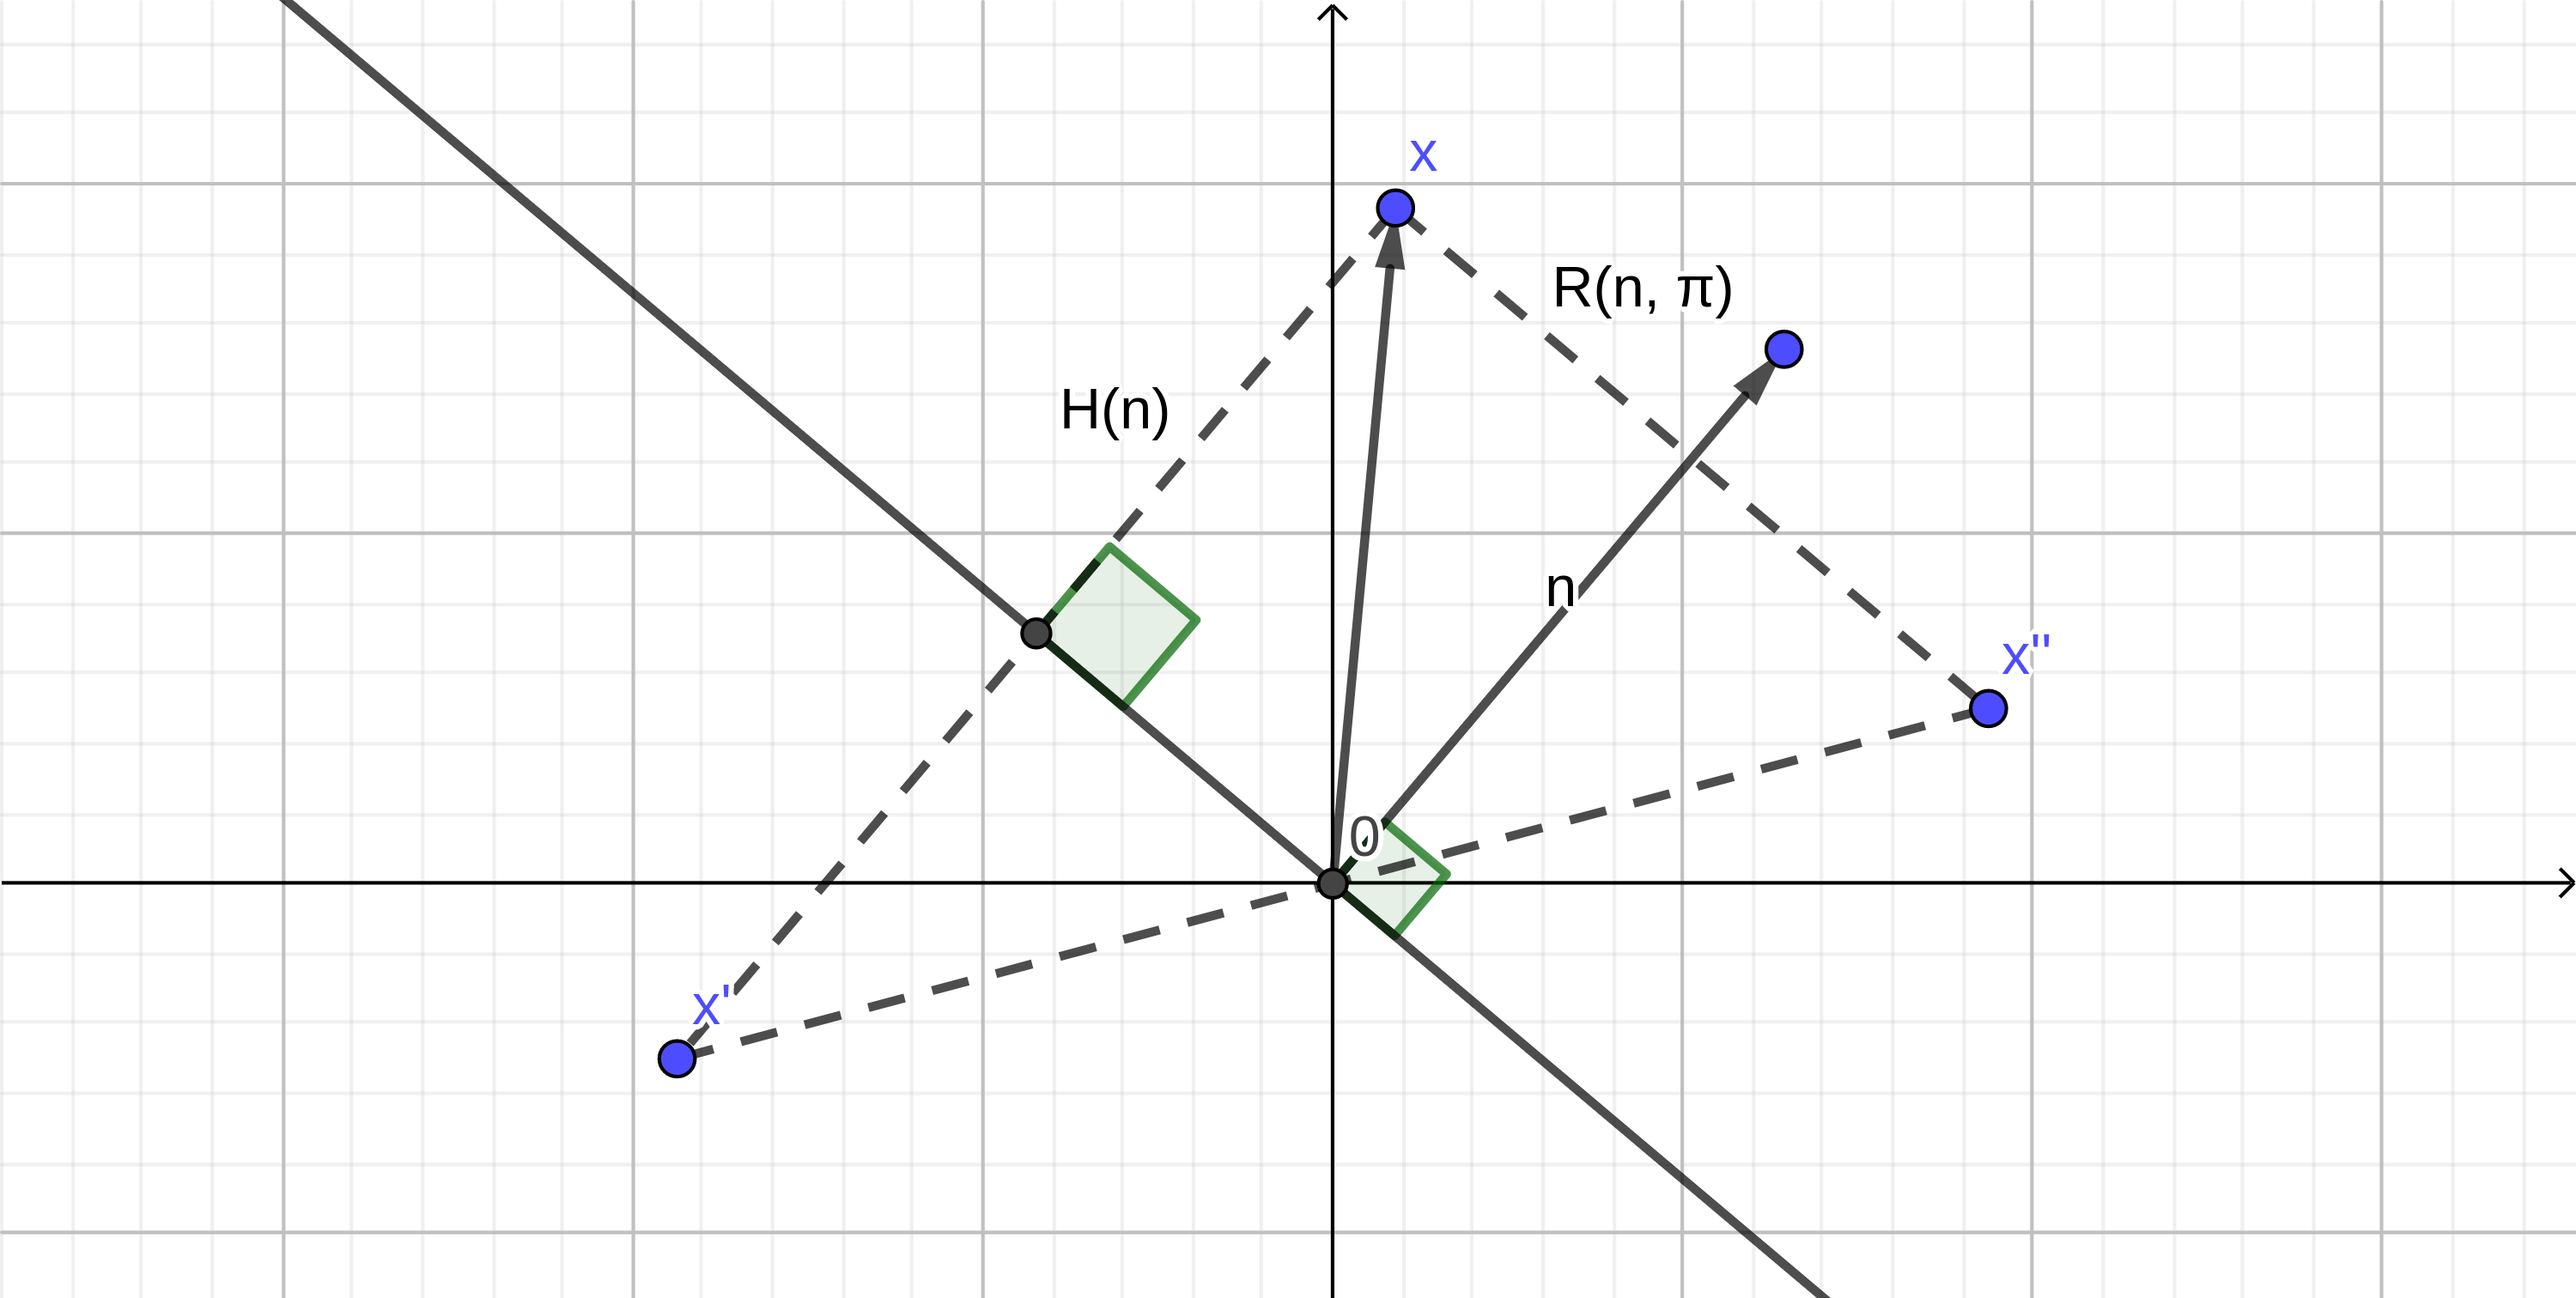
\includegraphics[width=0.5\textwidth]{q12_b.png}
       \end{center}
      \end{figure}
     \item First, explicitly find the matrix \(\mat H(\vec n)\):
      \begin{alignat*}2
       && \mat H(\vec n)_{ij} x_j = x_i' &= x_i - 2(\vec x \vecdot \vec n)n_i \\
       && &= \delta_{ij} x_j - 2 n_j n_i x_j \\
       \implies{}&& \mat H(\vec n)_{ij} &= \delta_{ij} - 2 n_i n_j
      \end{alignat*}
      Now
      \(\vec n_\pm
        = \cos(\frac 12 \theta)\,\vec i \pm \sin(\frac 12 \theta)\,\vec j\), so
      \begin{alignat*}2
       \mat H(\vec n_-)
        &={}&
        \begin{pmatrix}
         1 - 2\cos^2\tfrac 12\theta
          & \phantom{-{}} 2 \cos\tfrac 12\theta\sin\tfrac 12\theta
          & 0 \\[1ex]
         \phantom{-{}} 2 \cos\tfrac 12\theta\sin\tfrac 12\theta
          & 1 - 2\sin^2\tfrac 12\theta
          & 0 \\[1ex]
         0 & 0 & 1
        \end{pmatrix}
        &=
        \begin{pmatrix}
         -\cos\theta & \sin\theta & 0 \\
         \sin \theta & \cos\theta & 0 \\
         0 & 0 & 1
        \end{pmatrix} \\
       \mat H(\vec n_+)
        &={}&
        \begin{pmatrix}
         1 - 2\cos^2\tfrac 12\theta & -2 \cos\tfrac 12\theta\sin\tfrac 12\theta
          & 0 \\[1ex]
         -2 \cos\tfrac 12\theta\sin\tfrac 12\theta & 1 - 2\sin^2\tfrac 12\theta
          & 0 \\[1ex]
         0 & 0 & 1
        \end{pmatrix}
        &=
        \begin{pmatrix}
         -\cos\theta & -\sin\theta & 0 \\
         -\sin \theta & \cos\theta & 0 \\
         0 & 0 & 1
        \end{pmatrix} \\
       \mat H(\vec i)
        &=
        \mathrlap{
         \begin{pmatrix}
          -1 & 0 & 0 \\
          0 & 1 & 0 \\
          0 & 0 & 1
         \end{pmatrix}
        }
      \end{alignat*}
      and then
      \begin{equation*}
       \mat H(\vec i) \mat H(\vec n_-) =
        \mat H(\vec n_+) \mat H(\vec i)
         =
         \begin{pmatrix}
          \cos\theta & -\sin\theta & 0 \\
          \sin\theta & \cos\theta & 0 \\
          0 & 0 & 1
         \end{pmatrix}
         = \mat R(\vec k, \theta).
      \end{equation*}
      Geometrically, now just consider the components of \(\vec x\)
      in \(\vec i\) and \(\vec j\), as the component in
      \(\vec k\) is unaffected by \(\mat H(\vec n_\pm)\) and \(\mat H(\vec i)\).

      Then this result means that if we take some point \(x\), reflect it in the
      \(y\)-axis, reflect it in the line
      making a positive angle of \(\tfrac 12 \theta\) with the \(y\)-axis, then
      we get the same as if we had taken \(x\) and
      reflected it in the line making a negative angle of
      \(\frac 12 \theta\) with the \(y\)-axis and then reflected it in the
      \(y\)-axis, and both of these were in fact equivalent to rotating
      \(x\) by \(\theta\) about the origin (??)
      \begin{figure}[H]
       \begin{center}
       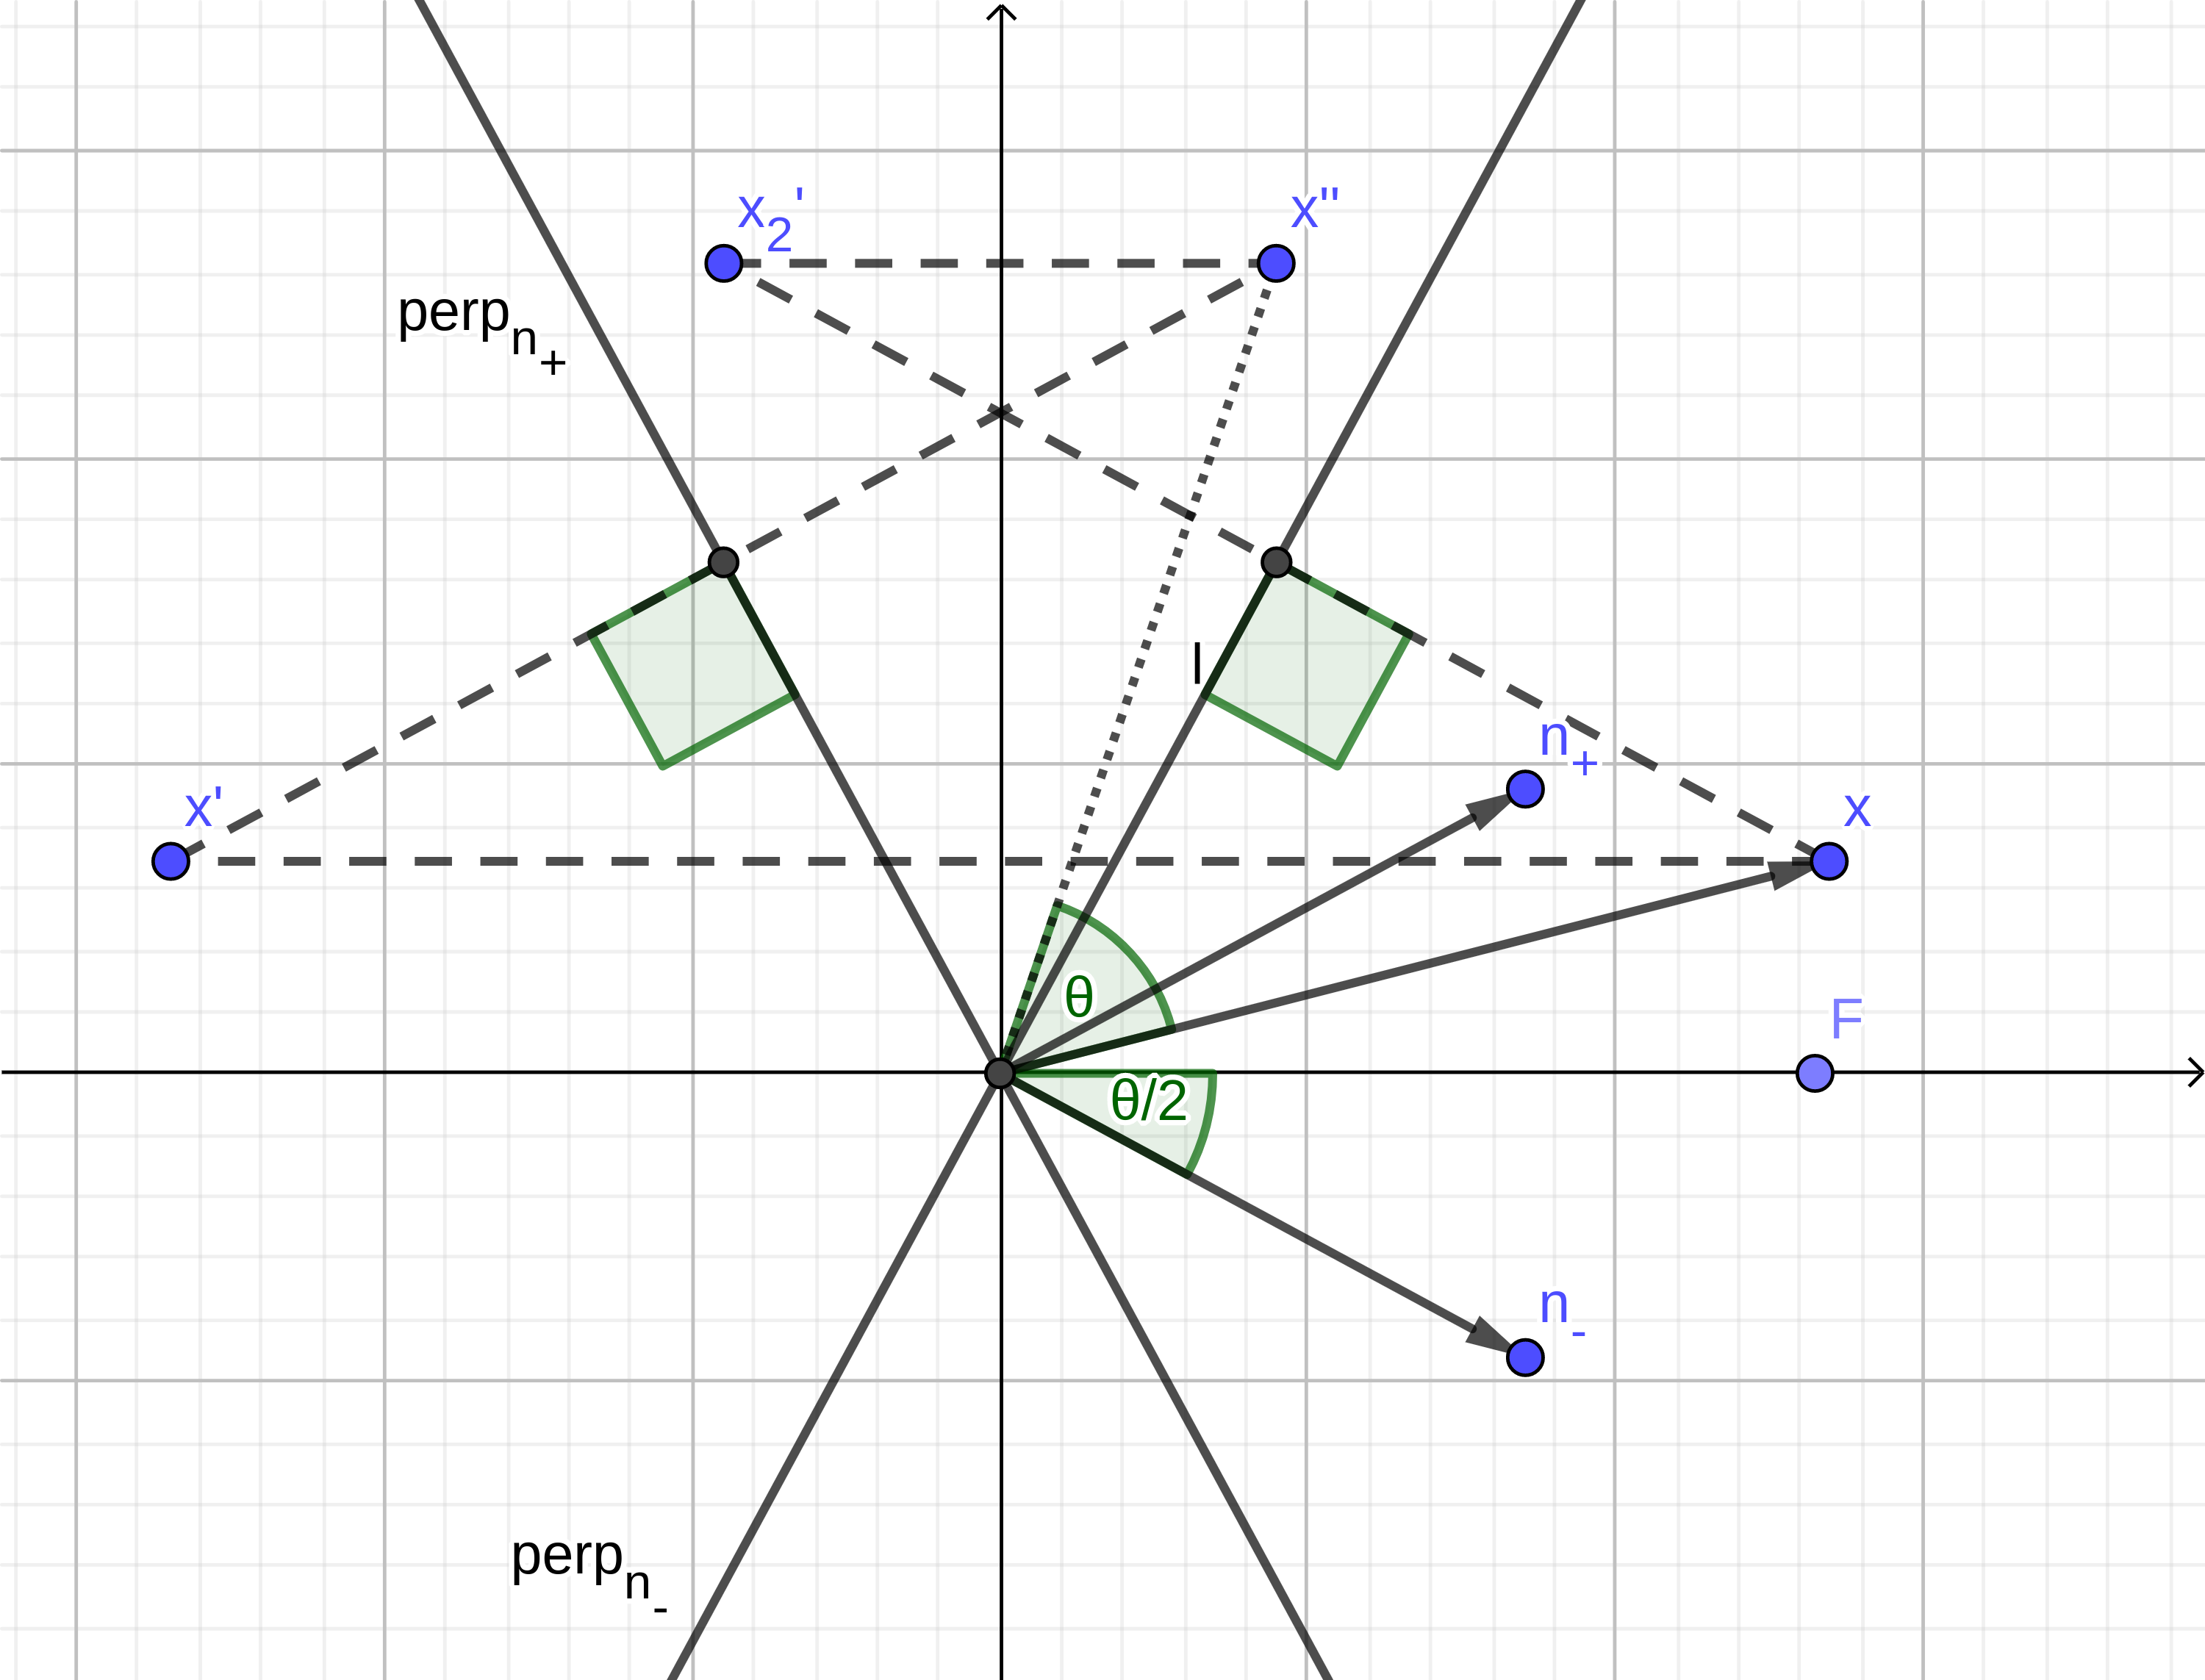
\includegraphics[width=0.5\textwidth]{12_c.png}
       \end{center}
      \end{figure}
    \end{enumerate}
 \end{enumerate}

\end{document}
